%%%%%%%% ICML 2019 EXAMPLE LATEX SUBMISSION FILE %%%%%%%%%%%%%%%%%

\documentclass{article}

% Recommended, but optional, packages for figures and better typesetting:
\usepackage{amsmath}
\usepackage{microtype}
\usepackage{graphicx}
\usepackage{subfigure}
\usepackage{booktabs} % for professional tables

% hyperref makes hyperlinks in the resulting PDF.
% If your build breaks (sometimes temporarily if a hyperlink spans a page)
% please comment out the following usepackage line and replace
% \usepackage{icml2019} with \usepackage[nohyperref]{icml2019} above.
\usepackage{hyperref}

% Attempt to make hyperref and algorithmic work together better:
\newcommand{\theHalgorithm}{\arabic{algorithm}}

% Use the following line for the initial blind version submitted for review:
\usepackage{icml2019}

% If accepted, instead use the following line for the camera-ready submission:
%\usepackage[accepted]{icml2019}

% The \icmltitle you define below is probably too long as a header.
% Therefore, a short form for the running title is supplied here:
\icmltitlerunning{Submission and Formatting Instructions for ICML 2019}

\begin{document}

\twocolumn[
\icmltitle{Deep Exploration via Stochastic Gradient Langevin Dynamic  \\
           in Deep Reinforcement Learning}

% It is OKAY to include author information, even for blind
% submissions: the style file will automatically remove it for you
% unless you've provided the [accepted] option to the icml2019
% package.

% List of affiliations: The first argument should be a (short)
% identifier you will use later to specify author affiliations
% Academic affiliations should list Department, University, City, Region, Country
% Industry affiliations should list Company, City, Region, Country

% You can specify symbols, otherwise they are numbered in order.
% Ideally, you should not use this facility. Affiliations will be numbered
% in order of appearance and this is the preferred way.
\icmlsetsymbol{equal}{*}

\begin{icmlauthorlist}
\icmlauthor{Jiantao Qiu}{thu}
\icmlauthor{Zhaoran Wang}{NU}
\icmlauthor{Yu Wang}{thu}
\end{icmlauthorlist}

\icmlaffiliation{thu}{Department of Electronic Engineering, University of Tsinghua University, Haidian, Beijing, China}
\icmlaffiliation{NU}{Industrial Engineering and Management Sciences, Northwestern University, Evanston, Illinois, USA}

\icmlcorrespondingauthor{Jiantao Qiu}{qjt15@mails.tsinghua.edu.cn}


% You may provide any keywords that you
% find helpful for describing your paper; these are used to populate
% the "keywords" metadata in the PDF but will not be shown in the document
\icmlkeywords{Deep exploration, Reinforcement learning}

\vskip 0.3in
]

% this must go after the closing bracket ] following \twocolumn[ ...

% This command actually creates the footnote in the first column
% listing the affiliations and the copyright notice.
% The command takes one argument, which is text to display at the start of the footnote.
% The \icmlEqualContribution command is standard text for equal contribution.
% Remove it (just {}) if you do not need this facility.

\printAffiliationsAndNotice{}  % leave blank if no need to mention equal contribution
%\printAffiliationsAndNotice{\icmlEqualContribution} % otherwise use the standard text.

\begin{abstract}
This document provides a basic paper template and submission guidelines.
Abstracts must be a single paragraph, ideally between 4--6 sentences long.
Gross violations will trigger corrections at the camera-ready phase.
\end{abstract}

\section{Introduction}
The application of deep neural networks in reinforcement learning has made appealing progress \cite{DQN,AlphaGO,OpenAIdota}. Deep neural networks serve as flexible function approximators, which enables reinforcement learning to solve various challenging tasks \cite{DQN,RN395}, e.g., the ones with pixel input using convolutional neural networks, and the ones that lack Markov property using recurrent neural networks. The latest generation of deep learning frameworks has convenient automatic derivation and integrates various optimizers \cite{PyTorch,MXNet,TF}. As in supervised learning,  ``loss function specification + stochastic gradient-based optimizer'' has become the standard approach to apply deep neural networks in reinforcement learning, both for Q-learning and policy gradient \cite{DDPG,DQN,PPO}.

However, in more difficult tasks, especially those with continuous state-action space and sparse or deceptive rewards, more effective exploration strategies become the key to success \cite{pnoise,colas2018gep}. In tasks with sparse rewards, unless a few specific events are triggered, the agent consistently witnesses zero rewards, which makes it necessary for the agent to traverse the policy space effectively, even without particular incentives \cite{VIME}. In tasks with deceptive rewards, due to the action penalty in the rewards, the agent consistently receives negative feedback during exploration, which renders the agent unable to explore and consequently choose to maintain the default action \cite{lehman2011abandoning,conti2018improving}. Such a situation makes it necessary for the agent to continue to explore the unknown part of the state-action space. Conversely, in the tasks with well-defined rewards, which can guide the agent to learn the optimal strategy, too much exploration may hurt the sample efficiency \cite{Showdown}. Such a trade-off between exploration and exploitation plays a vital role in reinforcement learning.

There has been a line of works on exploration strategies, including but not limited to random search (over action or parameter space) \cite{pnoise,DDPG}, count-based methods \cite{count1,count2}, and evolutionary strategies \cite{EPGRL,ERL2}. In particular, there is a class of exploration strategies based on Thompson sampling \cite{TS}, the core idea of which is to make greedy decisions based on the posterior distribution of value function. Thompson sampling has an ``instance-independent regret bound” \cite{TStutorial} and has been proven to be effective in a variety of deep reinforcement learning scenarios \cite{BDQN,VIME,dropoutInference,lastLayerBayes}.

However, when using deep neural networks to parametrize value functions, it is often intractable to calculate the posterior distributions in closed form. To address such a challenge, there has been a line of works on achieving posterior sampling through various approximation methods, including dropout \cite{dropoutInference}, variational inference \cite{VIME}, bootstrapping \cite{BDQN}, and so on. However, the posterior distributions obtained by these methods are often inaccurate, and moreover, may lack intrinsic motivation and suffer high computational cost \cite{osband2018randomized}.

Note that the optimization of value functions in reinforcement learning has many similarities with the optimization of loss functions in supervised learning. Such a key observation motivates us to use a stochastic gradient-based Monte Carlo sampler --- namely, Stochastic Gradient Langevin Dynamics (SGLD) --- to achieve posterior sampling \cite{SGLD}. In particular, we incorporate SGLD into the standard stochastic gradient-based optimizer to continuously generate posterior samples based on previously obtained observations. Then we use such samples to generate the actors for exploration during the rollout phase.

In this work, we use the Deep Deterministic Policy Gradient (DDPG) algorithm \cite{DDPG} as an example algorithm. Then we evaluate the performance of our exploration strategy with Continuous-Mountain-Car, Sparse-Half-Cheetah, and Half-Cheetah as deceptive, sparse, and well-defined tasks, and compare it against existing approaches based action noise and parameter noise. In general, the SGLD-based method can solve a broader variety of tasks with a single configuration. We summarize three major highlights of this work:
\begin{itemize}
\item  It is the first time to propose the use of SGLD to achieve Thompson sampling in the actor-critic algorithm, which uses deep neural networks as value functions.
\item We identify two difficulties of exploration: sparse reward and deceptive reward. The experimental results prove that our strategy can solve different difficult tasks with a single configuration.
\item  Our exploration strategy is application-friendly as it introduces no extra hyper-parameter, and has almost no additional computational overhead. 
\end{itemize} 

This paper is organized as follows: In Section 2, we analyze how the “zero reward” and “action penalty” issues in the environment affect the actor-critic algorithm and explore the works on relevant exploration strategies. Section 3 briefly introduces SGLD and explains how to use SGLD to sample critics following the posterior distribution, and how to incorporate exploration into the actor-critic algorithm. In Section 4, we implement SGLD-based exploration strategies using DDPG as a baseline algorithm and evaluate them in several different environments. Then the results are compared with the baseline, action noise, and parameter noise. Finally, we summarize this work in Section 5 and point out several future directions.

\section{Related works}
Reinforcement learning algorithms use neural networks as Q-value functions or policy functions achieve remarkable results in the continuous state-action space tasks . In order to solve more difficult tasks such as sparse or deceptive reward tasks, more effective exploration strategies have become a key point.

Some naive random search algorithms are generally used as default exploration strategies by various RL algorithms. Such as the $\epsilon$-greed method which takes non-optimal action according to probability $\epsilon$, or directly superimposes noise (correlation or not) in action space which called action space noise method. Another approach is to inject noise in the parameter space of the Q-value function of the policy function. In this situation, the agent will take the same action in the face of the same state within an episode, which leads to more consistent exploration behavior. However, such methods do not explicitly suggest how to use existing data to guide exploration, resulting in low sample efficiency. 

The Thompson sampling method, as a long-history exploration strategy, has recently returned to the perspective of deep reinforcement learning researchers. This method draws a sample from the posterior distribution of the Q-value function and makes decisions based on the random sample rather than an optimal estimation. Since it is difficult to directly calculate the posterior distribution of the neural network, the key point in the work of using Thompson sampling in reinforcement learning is the approach to achieve posterior sampling. For example, BDQN and prior-BDQN uses a multi-head network trained in bootstrapping way and treats the set of output as sampled results. VIME and SteinV PG use the reparameter trick and the stein gradient approach to implement variational inference as an approximation of the posterior distribution. These methods lack intrinsic motivation in the zero reward environment (Except prior-BDQN) and introduce considerable computational overhead. 

In this work, we use the SGLD to draw samples from the posterior distribution during training the value estimation function. There are a number of variants of SGLD, such as pre-condiction, SGHMC, SGFS, etc. The pre-condiction SGLD can be seen as a variant of RMSprop and has as almost equal number of operations, and been used as the sampler in this work. Because SGLD can be seen as accumulatng Gaussian noise during the optimization process, our method has similarities with parameter noise. The difference is that we add accumulated noise to the critic by SGLD, while they only add one-time noise to the actor when rollout samples. On the other hand, in prior-BDQN, they prepare a set of "prior function" in advance then select some of them to add on Q-value function during training, while in our algorithm there only have a single-head network with accumulated noise so that our method is more computational efficient.
\section{SGLD in Actor-Critic}
Under the Bayesian learning framework, there is one mathematical method that has both the "posterior sampling" and "parameter noise" properties, called stochastic gradient Langevin dynamics. In this section, we will briefly introduce the SGLD and show how it can be used to construct an exploration strategy in Actor-Critic algorithms.

\subsection{Stochastic Gradient Langevin Dynamic}
Stochastic Gradient Langevin Dynamic algorithm is an algorithm that can perform MCMC sampling by stochastic gradient descent + Gaussian noise \cite{SGLD}. For a paramter vector $\theta$ with a prior distribution $p(\theta)$ ,to draw a sample chain $\{\theta_1,\theta_2,\cdots\}$ follow $p(\theta|D)$ where $D=\{d_i\}^N_{i=1}$, the parameters should be updated as follow:
\begin{equation}
   \label{eq:sgld} 
   \begin{aligned}
\Delta\theta =\frac{\epsilon}{2}\frac{N}{n}\sum_{i=1}^{n}\nabla_\theta\log p(d_i|\theta)+\frac{\epsilon}{2}\nabla_\theta\log p(\theta)\\
+\mathcal{N}(0,\epsilon)
\end{aligned}
\end{equation}
Where $\epsilon$ is the learning rate, $n$ is the size of one mini-batch. 

The basic SGLD algorithm updates all parameters with the same step size, which leads to slow mixing rate. In practical, we use preconditioned SGLD (pSGLD) instead, in which the step size is scaled by preconditioner $G_t$ as follow:
\begin{equation}
   \label{eq:psgld} 
   \begin{aligned}
      \Delta\theta =\frac{\epsilon}{2}\frac{N}{n}G_t\sum_{i=1}^{n}\nabla_\theta\log p(d_i|\theta)+\frac{\epsilon}{2}G_t\nabla_\theta\log p(\theta)\\
      +\mathcal{N}(0,\epsilon G_t)
   \end{aligned}
\end{equation}
Where $G_t$ is updated as the mean square term in RMSprop \cite{rmsprop}.
\begin{figure*}[htbp]
   \begin{center}
      \centerline{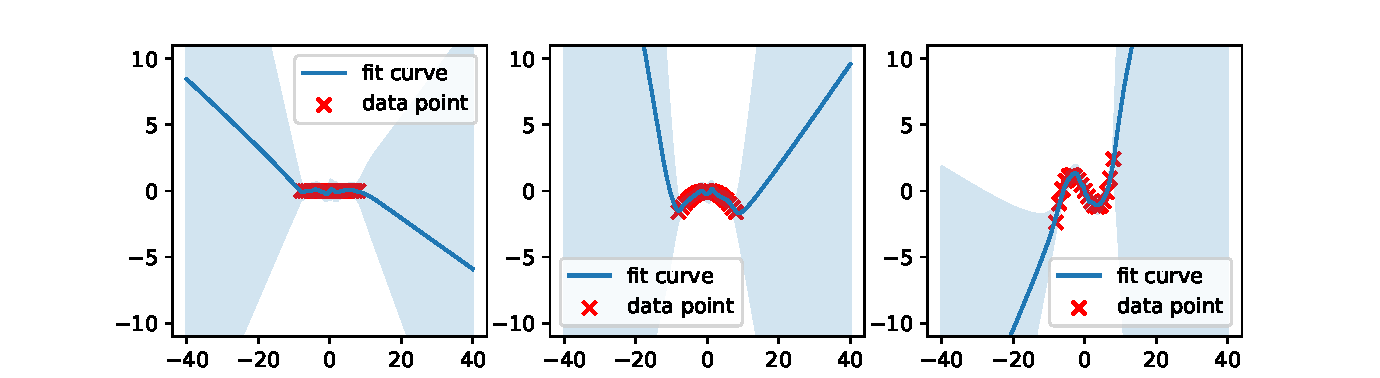
\includegraphics[width=480pt]{figs/three-curve}}
   \caption{The results of curve fitting by using pSGLD on three toy data sets.}
   \label{fig:three}
   \end{center}
\end{figure*}

%$\nabla_\theta p(d_i|\theta)$ is the data like-hood term, which corresponding to gradient of loss. $\nabla_\theta p(\theta)$ is prior probability term, it is equivalent to L2 regularization if $p(\theta)\sim\mathcal{N}(0,\sigma^2)$. And $\mathcal{N}(0,\epsilon)$ term make SGLD can sample parameters with $\theta \sim p(\theta|D)$
To visualize the ability of pSGLD to characterization the uncertainty of posterior distribution when fitting data set, we trained a neural network with architecture of "20-ReLU-20-ReLU-1" by pSGLD on three toy datasets, left: $y=0$, mid: $y=-x^2$, right: $y=x^3-x$, and the results are shown in the figure \ref{fig:three}. The dark curve is the average of the curve clusters, and the light areas represent the standard deviation of the curve clusters. The results show that the curve samples of pSGLD are concentrated near the data points, while diverge in both positive and negative directions in areas far from the data, even on the all zero data set.

\subsection{Posterior sampling of critic}
\label{sec:samplecritic}
In Deep Actor Critic algorithm, the parameters of critic network $\theta^Q$ is updated by an SGD-like optimizer to minimize the MSE error $L^Q=\sum(R-V(S|\theta^Q))$. To replace the SGD-like optimizer by pSGLD sampler with minimal changes, we suppose that the likelihood term is $p(d_i|\theta^Q)\sim\exp(-L^Q)$ to match the Bellman error, and prior term is $p(\theta^Q)\sim \mathcal{N}(0,\sigma^2)$ to match the L2 regularization on critic network. Then the critic will updated as follow :
\begin{equation}
   \label{eq:rlpsgld} 
   \begin{aligned}
      \Delta\theta^Q =-\frac{\epsilon}{2}\frac{N}{n}G_t\sum_{i=1}^{n}\nabla_\theta L^Q -\frac{\epsilon}{2}G_t \frac{\theta^Q}{\sigma^2}\\
      +\mathcal{N}(0,\epsilon G_t)
   \end{aligned}
\end{equation}
It is worth noting that, for off-policy algorithm with replay buffer, the size of data sets $N$ in reinforcement learning is increasing as the training process increases. If the learning rate $\epsilon$ remains constant, the gradient of the likelihood term will continue to grow, resulting in an unstable training process. In order to keep the training process stable, we implement learning rate decay as opposed to data set size growth: $\epsilon_t=\frac{n}{N}\epsilon_0$. Now the equation (\ref{eq:rlpsgld}) turns into:
\begin{equation}
   \label{eq:rlpsgld1} 
   \begin{aligned}
      \Delta\theta^Q =-\frac{\epsilon_0}{2}G_t\sum_{i=1}^{n}\nabla_\theta L^Q -\frac{\epsilon_0}{2}\frac{n}{N}G_t \frac{\theta^Q}{\sigma^2}\\
      +\mathcal{N}(0,\epsilon_0\frac{n}{N} G_t)
   \end{aligned}
\end{equation}
The observed data is increasing as the learning process progresses, which leads to the effect of the prior term and the noise term becomes weaker than the likelihood term. This is consistent with our common sense: the more data is observed, the more the model's distribution is concentrated toward the maximum likelihood estimate.
\begin{algorithm}[htbp]
   \caption{Deep Actor Critic with SGLD}
   \label{alg:sgldac}
\begin{algorithmic}
   \STATE {\bfseries Input:} environment $E$, critic $V(s|\theta^V)$, actor $\pi(s|\theta^\pi)$, exploration strategy $\tilde\pi \leftarrow f(\pi)$
   \FOR{1 {\bfseries to} cycle\_number}
   \STATE Copy the actor for rollout $\tilde \pi\leftarrow \pi$
   \FOR{1 {\bfseries to} rollout\_update\_number}
   \STATE Update $\tilde\pi$ by policy gradient with last critic.
   \ENDFOR
   \STATE Rollout data $\{d_t\}$ from $E$ by $\tilde\pi$
   \FOR{1 {\bfseries to} update\_number}
   \STATE Sample Critic $V(s|\theta^V) \sim p(\theta^V|D)$ with SGLD
   \STATE Update Actor $\pi(s|\theta^\pi)$ by policy gradient 
   \ENDFOR
   \ENDFOR
\end{algorithmic}
\end{algorithm}
\subsection{Exploration for Actor-Critic Algorithm}
The Actor-Critic algorithm using SLGD is shown in algoritm \ref{alg:sgldac}. Critic $V(s|\theta^V)$ is continuously sampled by SGLD, so the last critic in the network is a sample follow $p(\theta^V|D)$ at any time. In the rollout phase, the current actor $\pi$ is copied to $\tilde\pi$, then update $\tilde\pi$ use the policy gradient generated by the last critic. In Actor-Critic algorithm, the critic does not make decisions directly, so we optimize the copy of current actor with the last critic sample to get the optimal strategy of the last critic. We do this to follow the principle of Thompson sampling: making decisions based on the sampled value prediction model. The policy gradient with posterior sampled critic can estimated follow equation \ref{eq:acpg}, which similar as \cite{dropoutInference}.
\begin{equation}
   \label{eq:acpg} 
   \begin{aligned}
   \nabla_{\theta^\pi}\mathbb{E}[L^\mu|D] = \mathbb{E}_{s_t\sim\rho,a_t\sim\pi,\theta^V\sim p(\theta^V|D)}[\nabla_{\theta^\pi}L^\pi]\\
   \end{aligned}
\end{equation}
Now we confirm the sanity check as \cite{osband2018randomized} one by one: \textbf{Posterior Concentration}: As described in section \ref{sec:samplecritic}, the intensity of the noise term and prior term will be weaker as more data is observed, and the distribution of critic will concentrate to the most likelihood estimation. \textbf{Multi-step Uncertainty}: The uncertainty of critic will be propagated throught the bootstrap value estimation target $R$. \textbf{Epistemic vs Aleatoric}: The SGLD sampler does posterior sampling follow $p(\theta^V|D)$ instead of $p(r_t|s_t,a_T)$. \textbf{Task-appropriate}: The SGLD sampler does posterior sampling in parameter space instead of state-action space which related to the environment. \textbf{Intrinsic motivation}: Even in zero reward environment, the SGLD sampler can give non-zero value estimation on unseen states. These analysis demonstrate that SGLD based exploration strategy can effectively overcome the shortcomings of existing exploration strategies.
\section{Results and Discussion}
\subsection{Experiment setting}
We choose MontainCar\_continous(MC) as a deceptive reward task, SparseHalfCheetah(SHC) as a sparse reward task,and HalfCheetah(HC) as well defined task.

We use Ubuntu16.04 on XX CPU+XX GPU. We use gym XX + mujoco 1.5.1
\subsection{Sample critic with uncertainty}
We rollout some transitions in MC, and plot the state point in "position-velocity". Then we train a critic network with these data by Adam optimizer and SGLD sampler. In both cases we start with an random initialized network and pre-train the critic network for XX steps to make sure convergence. After preparation, we further optimize the network for XX steps, and store the copy of critic network after each optimize step as one sample. BalaBala....

We can see SGLD can sample critic which have high uncertainty on the periphery state domain.

\subsection{Exploration in sparse or deceptive tasks}

We compared the effects of various exploration methods on the MC and SHC tasks.

\subsection{Exploration in well defined tasks}

We compared the effects of various exploration methods on the HC task.


\section{Conclusion and Further work}
This article summarizes the reasons that lead to difficulties in exploring sparse/depetive tasks as "zero reward" and "action penalty" and indicates how these factors affect reinforcement learning algorithms. We propose an exploring strategies using SGLD to achieve Tompson sampling in Actor-critic algorithm, which overcomes the shortcomings of existing algorithms and achieve effectively explore in sparse/deceptive tasks, with no additional hyperparameters are introduced and is computationally friendly. We use the same settings to evaluate our method on three continous tasks, and the results show that our method can solve more tasks and the sample is more efficient.

Our work demonstrates the exploration strategy with combination of parameter noise and posterior sampling in reinforcement learning. This algorithm continuously generates the sampling of the value function under all observed data and the corresponding policy during the training process. This approach may be combined with evolution algorithms as a way to generate new populations, which may cause cover the policy parameter space better and make full use of the data for each time step. In addition, the intensity of exploration in our approach is related to the number of data observed, which means throwing away some of the redundant data will "restart" the exploration, combined with further data management strategy design may lead to better exploration.


% In the unusual situation where you want a paper to appear in the
% references without citing it in the main text, use \nocite
%\nocite{langley00}

\bibliography{reference}
\bibliographystyle{icml2019}


\end{document}


% This document was modified from the file originally made available by
% Pat Langley and Andrea Danyluk for ICML-2K. This version was created
% by Iain Murray in 2018, and modified by Alexandre Bouchard in
% 2019. Previous contributors include Dan Roy, Lise Getoor and Tobias
% Scheffer, which was slightly modified from the 2010 version by
% Thorsten Joachims & Johannes Fuernkranz, slightly modified from the
% 2009 version by Kiri Wagstaff and Sam Roweis's 2008 version, which is
% slightly modified from Prasad Tadepalli's 2007 version which is a
% lightly changed version of the previous year's version by Andrew
% Moore, which was in turn edited from those of Kristian Kersting and
% Codrina Lauth. Alex Smola contributed to the algorithmic style files.
